\documentclass[10pt]{beamer}

\usepackage[english]{babel}
\usepackage[utf8]{inputenc}
\usepackage[T1]{fontenc}
\usepackage{lmodern}

\usepackage{layout}
%\usepackage{epsfig}
\usepackage{graphicx}
\graphicspath{{../rapport/images/}}
\usepackage[outdir=../rapport/images/]{epstopdf}
\usepackage{subfigure}
\usepackage{tikz}
\usepackage{numprint}


\usepackage{siunitx}
\usepackage{eurosym}

\usepackage{amsthm}
\usepackage{amsmath}
\usepackage{amssymb}

\usepackage{mathrsfs}
\usepackage{wrapfig}
\usepackage{url}
\usepackage{multirow}
\usepackage{array}
\usepackage{pgfplots}

\usepackage[version=3]{mhchem}

\usepackage{wasysym}
%Bibtex
%\usepackage[square]{natbib}
%\newcommand{\newblock}{}

\usetheme{Warsaw}
\setbeamertemplate{headline}{}

\usepackage{graphicx}
\usepackage{epsfig}
%\usepackage{epstopdf}

\makeatletter
\newcommand*{\rom}[1]{\expandafter\@slowromancap\romannumeral #1@}
\makeatother

\usepackage{todonotes}
\title{Multi-characteristics reputation system using iterative filtering}
\author[Malian DR, Quentin L]{
  \small
  Malian De Ron
 \and
  Quentin Laurent
}

\begin{document}

\begin{frame}
  \maketitle
\end{frame}
\begin{frame}
\frametitle{Method for $N$ judges, $M$ objects and $K$ characteristics}
\begin{block}{Components}
\begin{itemize}
\item Ratings tensor : $X \in \mathbb{R}^{N\times M \times K}$
\item Reputation tensor : $R \in \mathbb{R}^{M\times K}$
\item Weight vector : $w \in \mathbb{R}^{N\times 1}$
\end{itemize}
\end{block}
\begin{block}{Two stages of the method}
\begin{itemize}
\item Preprocessing : possibly center the votes to zero and set variances to 1.
\item Iteration : determine weights of the judges and the final reputation
\end{itemize}
\end{block}
\end{frame}

\begin{frame}
\begin{block}{Two steps iteration}
\begin{itemize}
\item Reputation computation : weighted sum of the votes
$$R_{jk}^{t+1}(w,X) = \frac{\sum_{i}X_{ijk}w^t_{i}}{\sum_i w_{i}}$$
\item Filtering : The farther a judge $i$ rates from the reputation, the lesser its weight\\
Define the column vector $d^{ij} \in \mathbb{R}^K$ as follows :
$$ d^{ij}_k = X_{ijk}-R^{t+1}_{jk}$$
$$div_i =  \frac{1}{MK}\sum_{j} (d^{ij})^T (d^{ij})$$
$$w_i^{t+1}(X,r) = 1 -k \cdot div_i$$
with $k$ a constant 
\end{itemize}
\end{block}
\end{frame}
\begin{frame}
\frametitle{Example for one judge and one object for $K=2$}
\begin{block}{}
Weight according to $d^{ij}\in \mathbb{R}^{2\times 1}$
\begin{figure}
\centering
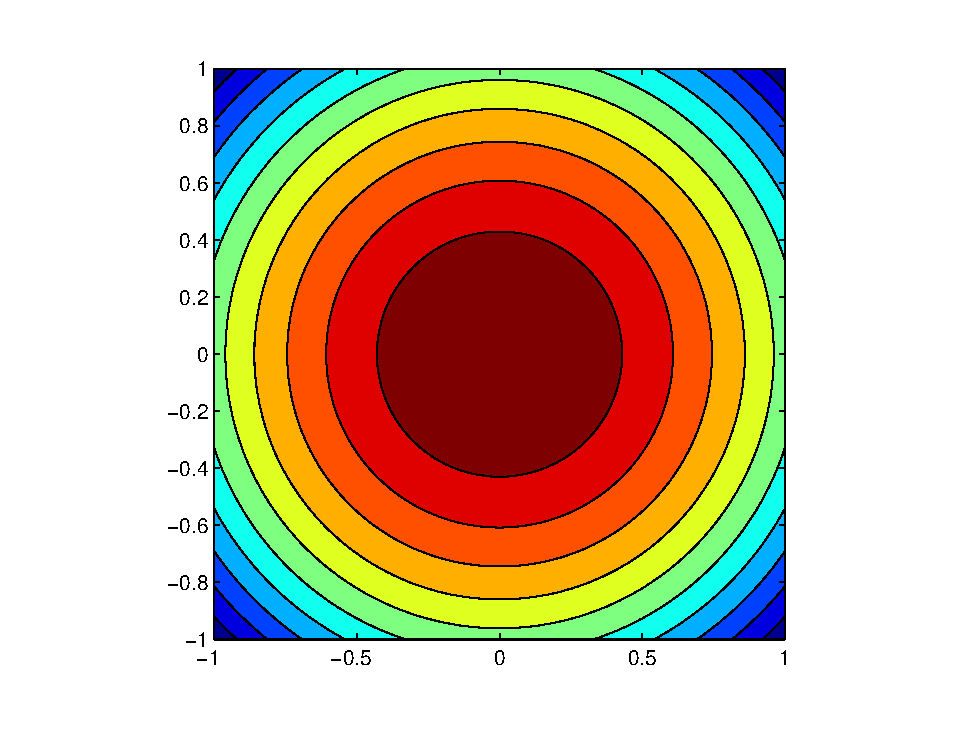
\includegraphics[width = 7cm]{../rapport/images/courbes.eps}
\end{figure}
We simply take the sum of this over all the objects
\end{block}
\end{frame}

\begin{frame}
\frametitle{Properties of the method}
\begin{block}{Energy function}
\begin{itemize}
\item Fix points of the iteration are stationary points of the energy function
$$E(r) =  \sum_{i=1}^n \int_0^{div_i(r)}g(u) du + c $$
\item The stationary point in the domain concerned is unique and is a strict minimum
\item The iteration corresponds to a steepest descent method step
\end{itemize}
\end{block}
\end{frame}
\definecolor{applegreen}{rgb}{0.55, 0.71, 0.0}
\definecolor{airforceblue}{rgb}{0.36, 0.54, 0.66}

\begin{frame}
  \frametitle{Simple example}
  \begin{block}{$N \times M \times K = 3$ juges $ \times$ 2 teams $\times$ 2 characteristics}
  \begin{center}
$
X(:, : ,1) = \overbrace{
    \begin{pmatrix}
    4.2 & 3.4 \\ 
    4.5 & 3.3 \\ 
    2.8 & 4.9
    \end{pmatrix} 
}^{\text{Artistic skill}}
$
\qquad\qquad
$
X(:, :, 2) = 
\underbrace{
    \begin{pmatrix}
    4.3 & 3.3 \\ 
    4.4 & 3.4 \\ 
    2.8 & 4.8
    \end{pmatrix} 
}_{\text{Technical skill}}
$
  \end{center}
  \end{block}
\end{frame}

\begin{frame}
  \frametitle{Simple example}
  \begin{block}{$N \times M \times K = 3$ juges $ \times$ 2 teams $\times$ 2 characteristics}
  \begin{center}
$
X(:, : ,1) = \overbrace{
    \begin{pmatrix}
    4.2 & 3.4 \\ 
    4.5 & 3.3 \\ 
    \textcolor{red}{2.8} & \textcolor{applegreen}{4.9}
    \end{pmatrix} 
}^{\text{Artistic skill}}
$
\qquad\qquad
$
X(:, :, 2) = 
\underbrace{
    \begin{pmatrix}
    4.3 & 3.3 \\ 
    4.4 & 3.4 \\ 
    \textcolor{red}{2.8} & \textcolor{applegreen}{4.8}
    \end{pmatrix} 
}_{\text{Technical skill}}
$
  \end{center}
  \end{block}
\end{frame}

\begin{frame}
  \frametitle{Simple example: simple mean}
    \begin{block}{Vector of Reputation $R^{M \times K} = R^{ \text{ 2 teams } \times  \text{ 2 characteristics}}$}
  \begin{center}
$
    \begin{pmatrix}
    3.83 & \textcolor{applegreen}{3.87} \\ 
    \textcolor{airforceblue}{3.83} & \textcolor{airforceblue}{3.83}
    \end{pmatrix} 
$
  \end{center}
  \end{block}
  
  Who's winning? The favored team

    \begin{block}{Mean of mean}
  \begin{center}
$
    \begin{pmatrix}
    \textcolor{red}{3.83} & \textcolor{applegreen}{3.85}
    \end{pmatrix} 
$
  \end{center}
  \end{block}

\end{frame}

\begin{frame}
  \frametitle{Simple example: Iterate}
    \begin{block}{Vector of Reputation $R^{M \times K} = R^{ \text{ 2 teams } \times  \text{ 2 characteristics}}$}
  \begin{center}
$
    \begin{pmatrix}
    \textcolor{applegreen}{4.07} & \textcolor{red}{3.63} \\ 
    \textcolor{applegreen}{4.07} & \textcolor{red}{3.61}
    \end{pmatrix} 
$
  \end{center}
  \end{block}
  
  Who's winning? The first team

    \begin{block}{Mean of mean}
  \begin{center}
$
    \begin{pmatrix}
    \textcolor{applegreen}{4.07} & \textcolor{red}{3.62}
    \end{pmatrix} 
$
  \end{center}
  \end{block}

\end{frame}


\begin{frame}
  \frametitle{Simple example: Separated}
    \begin{block}{Vector of Reputation $R^{M \times K} = R^{ \text{ 2 teams } \times  \text{ 2 characteristics}}$}
  \begin{center}
$
    \begin{pmatrix}
    \textcolor{applegreen}{3.86} & \textcolor{red}{3.83} \\ 
    \textcolor{applegreen}{3.86} & \textcolor{red}{3.8}
    \end{pmatrix} 
$
  \end{center}
  \end{block}
  
  Who's winning? The first team

    \begin{block}{Mean of mean}
  \begin{center}
$
    \begin{pmatrix}
    \textcolor{applegreen}{3.86} & \textcolor{red}{3.82}
    \end{pmatrix} 
$
  \end{center}
  \end{block}

\end{frame}

\begin{frame}
  \frametitle{Improvements}
  \begin{itemize}
      \item N judges, M objects, K characteristics and P points of view !
      \item Weight the importance of notes
      \item Analyze different cheating behavior
      \item Apply the algorithm on student 
  \end{itemize}


\end{frame}



\end{document}
